\subsubsection{Finite Element Meshes}

This section reports the finite element meshes employed in the numerical simulations,
including both the analytical spherical benchmark and the full phantom--head geometry.
Figures~\ref{fig:phantom_mesh} and~\ref{fig:sphere_mesh} show the corresponding meshes,
and Table~\ref{tab:mesh_comparison} summarizes global mesh statistics and quality indicators.

\begin{figure}[htbp]
    \centering
    \begin{subfigure}[t]{0.43\textwidth}
        \centering
        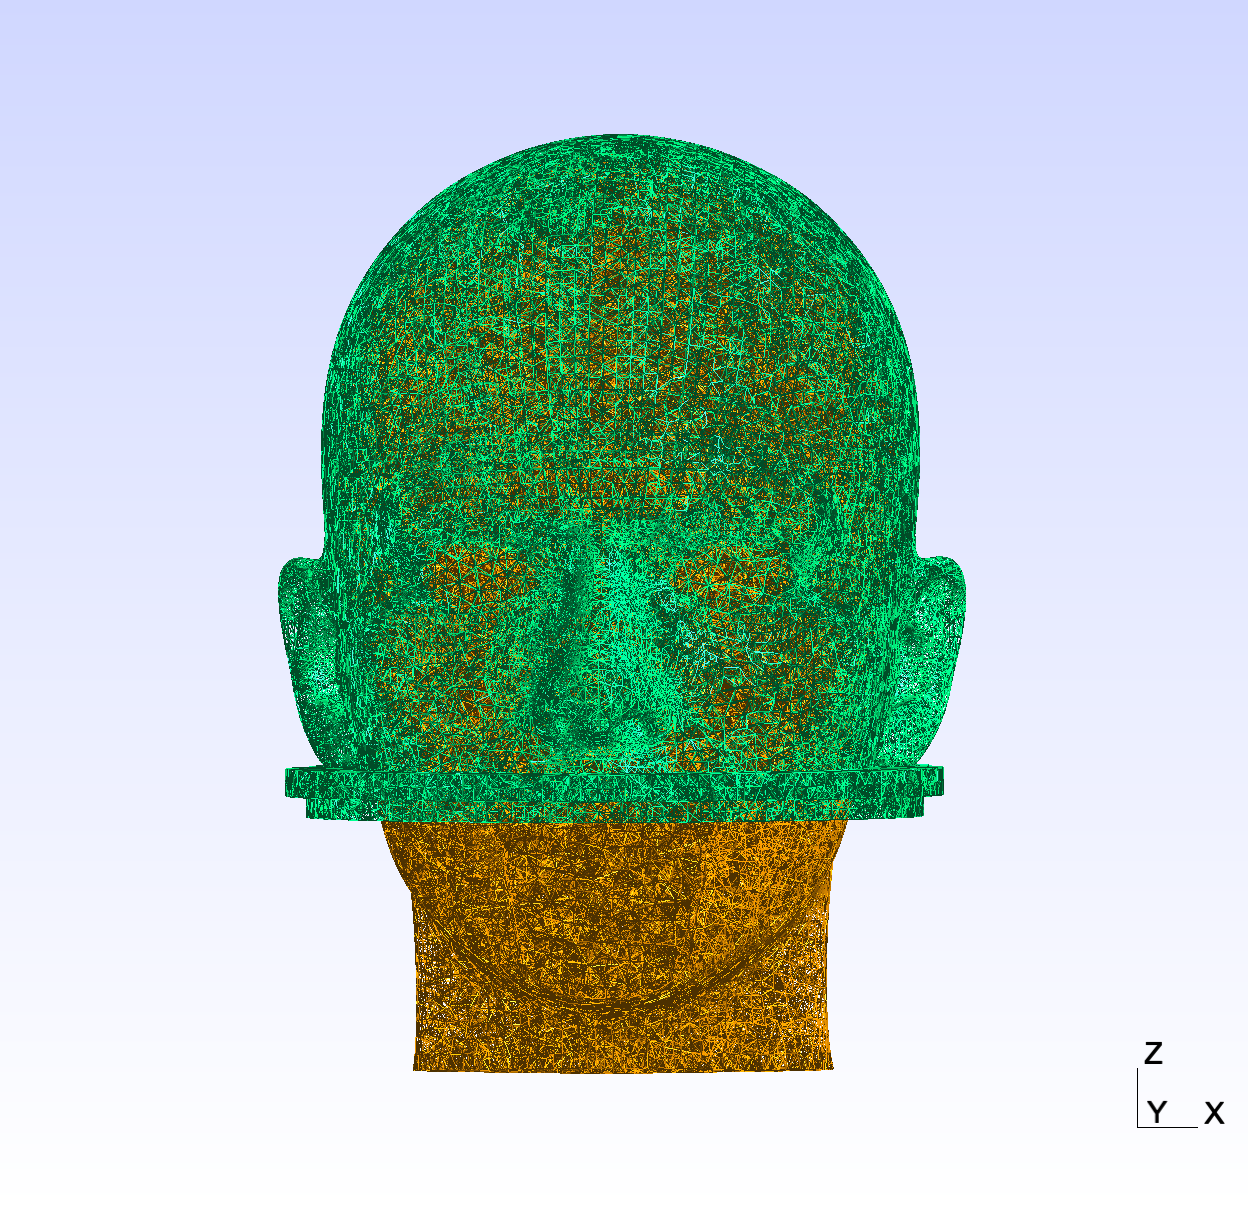
\includegraphics[width=\textwidth]{../../02_Images/phantom-head-mesh-frontal.png}
        \caption{Frontal view}
        \label{fig:phantom_mesh_frontal}
    \end{subfigure}
    \hfill
    \begin{subfigure}[t]{0.43\textwidth}
        \centering
        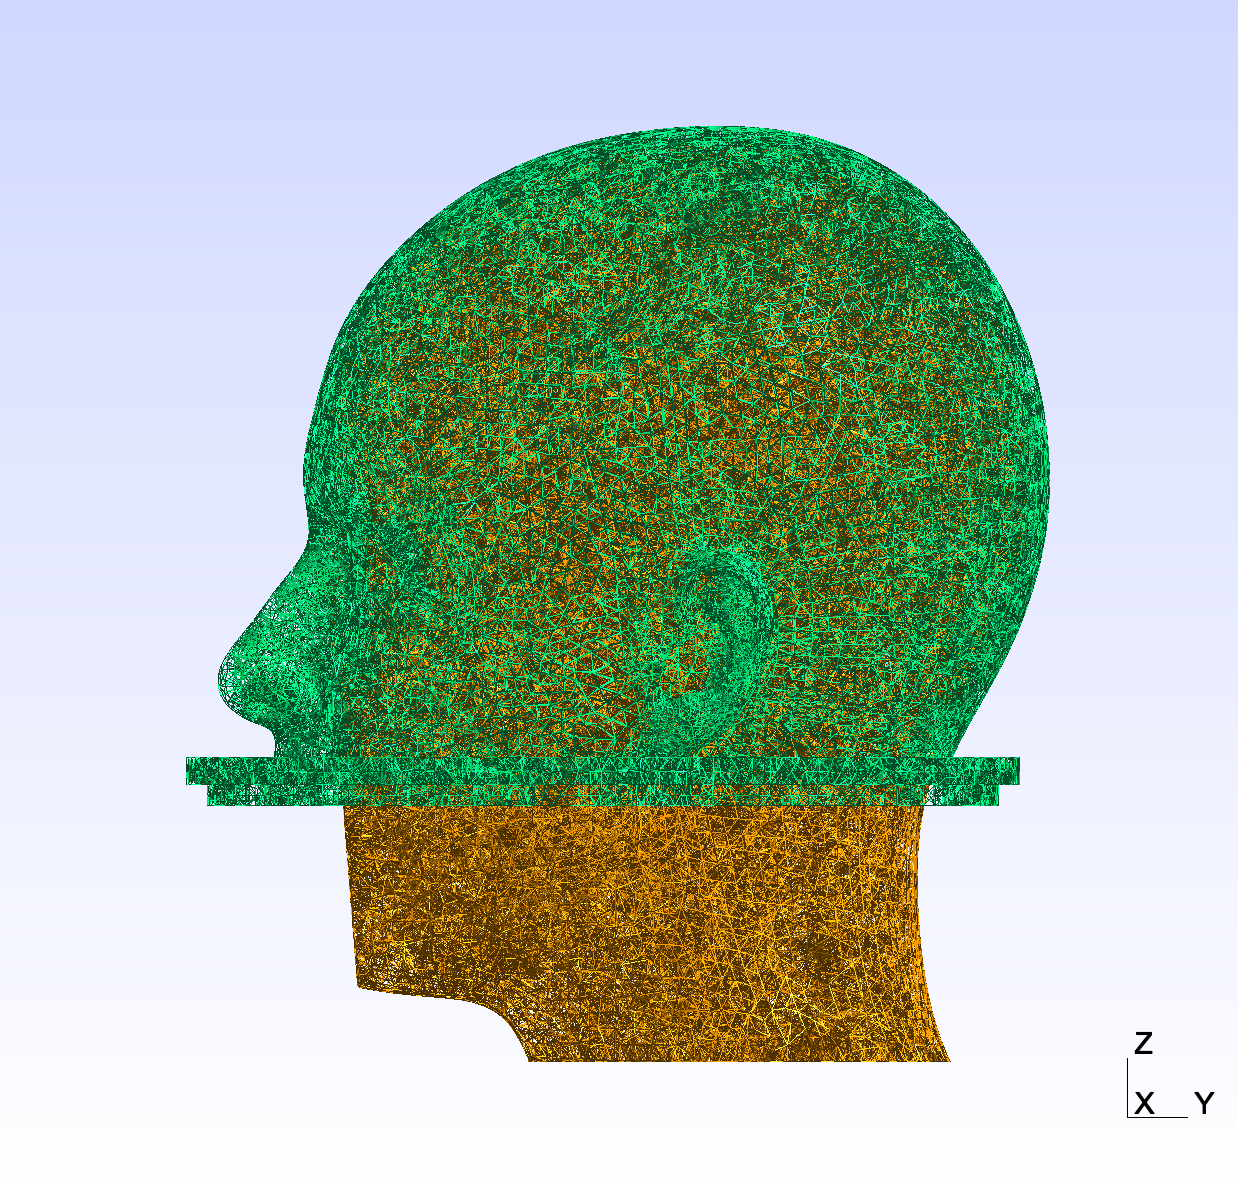
\includegraphics[width=\textwidth]{../../02_Images/phantom-head-mesh-lateral.png}
        \caption{Lateral view}
        \label{fig:phantom_mesh_lateral}
    \end{subfigure}
    \caption[Phantom head mesh]{
    Finite element mesh of the phantom--head geometry.
    }
    \label{fig:phantom_mesh}
\end{figure}

\begin{figure}[htbp]
    \centering
    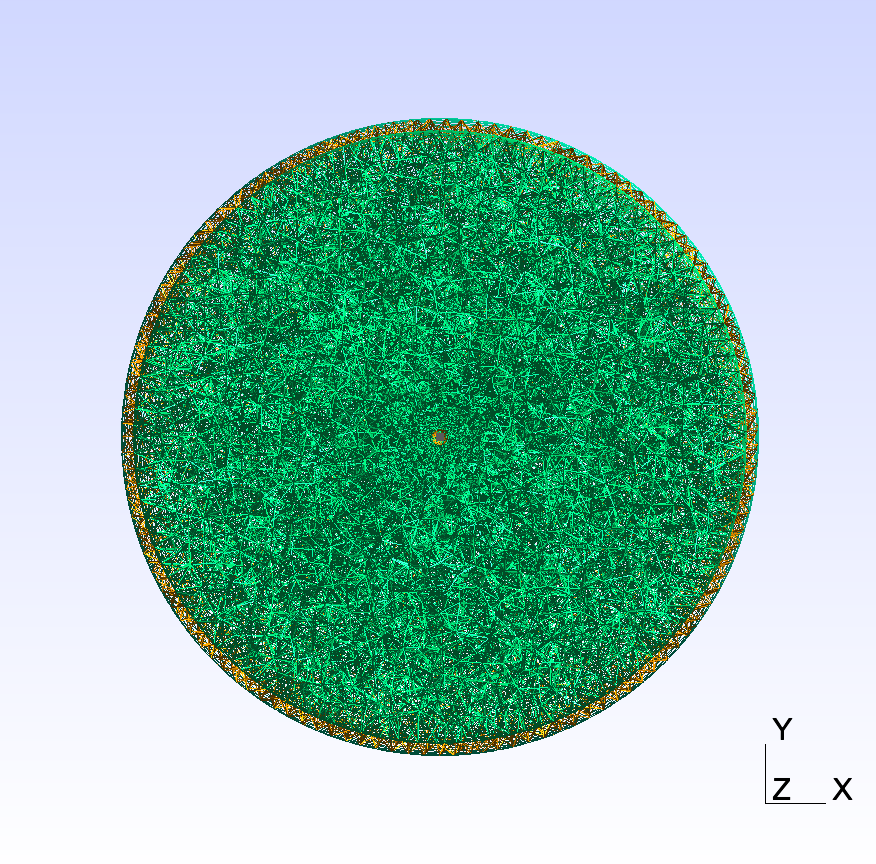
\includegraphics[width=0.5\textwidth]{../../02_Images/sphere-mesh.png}
    \caption[Spherical benchmark mesh]{
    Finite element mesh of the concentric spherical benchmark geometry.
    }
    \label{fig:sphere_mesh}
\end{figure}

\begin{table}[htbp]
\centering
\caption[Mesh statistics comparison]{Comparison of mesh statistics and quality indicators
for the spherical benchmark and phantom--head numerical models.}
\label{tab:mesh_comparison}
\small
\begin{tabularx}{\textwidth}{l X X}
\toprule
\textbf{Metric}
& \textbf{Spherical Benchmark}
& \textbf{Phantom Head Model} \\
\midrule
Total nodes
& $2.47 \times 10^{5}$
& $1.95 \times 10^{6}$ \\[3pt]

Tetrahedral elements
& $1.80 \times 10^{5}$
& $1.40 \times 10^{6}$ \\[3pt]

Surface triangles
& $1.70 \times 10^{4}$
& $1.95 \times 10^{4}$ \\[3pt]

SICN
& $0.82\,(-0.72,\;0.999)$
& $0.80\,(-0.54,\;1.00)$ \\[3pt]

Gamma
& $0.80\,(0.14,\;0.99)$
& $0.77\,(6.7\times10^{-7},\;1.00)$ \\[3pt]

SIGE
& $0.84\,(-0.73,\;0.98)$
& $0.82\,(-0.70,\;1.00)$ \\

\bottomrule
\end{tabularx}
\end{table}
